\begin{longtable}{|r l|p{2cm}|p{6cm}|p{2cm}|}
\hline
\multicolumn{2}{|c|}{Requisito} & Tipologia & Descrizione & Fonti\tabularnewline
\hline
 & \hypertarget{R-3V1}{R-3V1} & Vincolo

Obbligatorio & La parte destinata ai creatori di domande e di questionari dovrà essere fruibile attraverso un PC & Capitolato\tabularnewline
\hline
 & \hypertarget{R-3V2}{R-3V2} & Vincolo

Obbligatorio & La parte server deve essere realizzata in Javascript con server node.js
 & Capitolato\tabularnewline
\hline
 & \hypertarget{R-3V3}{R-3V3} & Vincolo

Obbligatorio & La parte client dovrà essere eseguibile in un browser HTML5 & Capitolato\tabularnewline
\hline
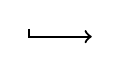
\begin{tikzpicture}
\draw [->, thick] (0.2,0.2) -- (0.2,0.1) -- (1,0.1);
\end{tikzpicture} & \hypertarget{R-3V3.1}{R-3V3.1} & Vincolo

Obbligatorio & L'applicazione funziona correttamente su Chrome versione 47.0.2526 e successive & Capitolato\tabularnewline
\hline
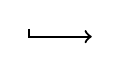
\begin{tikzpicture}
\draw [->, thick] (0.2,0.2) -- (0.2,0.1) -- (1,0.1);
\end{tikzpicture} & \hypertarget{R-3V3.2}{R-3V3.2} & Vincolo

Obbligatorio & L'applicazione funziona correttamente su Firefox versione 38.5.2esr e successive & Capitolato\tabularnewline
\hline
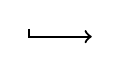
\begin{tikzpicture}
\draw [->, thick] (0.2,0.2) -- (0.2,0.1) -- (1,0.1);
\end{tikzpicture} & \hypertarget{R-3V3.3}{R-3V3.3} & Vincolo

Obbligatorio & L'applicazione funziona correttamente su Microsoft Edge versione 25.10586 e successive & Capitolato\tabularnewline
\hline
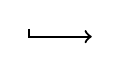
\begin{tikzpicture}
\draw [->, thick] (0.2,0.2) -- (0.2,0.1) -- (1,0.1);
\end{tikzpicture} & \hypertarget{R-3V3.4}{R-3V3.4} & Vincolo

Obbligatorio & L'applicazione funziona correttamente su Safari versione 9.0.2 e successive & Capitolato\tabularnewline
\hline
 & \hypertarget{R-3V4}{R-3V4} & Vincolo

Obbligatorio & L'applicazione deve utilizzare fogli stile CSS3 per l’ aspetto estetico & Capitolato\tabularnewline
\hline
 & \hypertarget{R-3V5}{R-3V5} & Vincolo

Obbligatorio & L'applicazione deve utilizzare Javascript per la parte attiva del client & Capitolato\tabularnewline
\hline
 & \hypertarget{R-3V6}{R-3V6} & Vincolo

Obbligatorio & La parte destinata agli esaminandi dovrà funzionare con qualunque dispositivo: dal Personal Computer, ai Tablet ed agli SmartPhone attraverso browser & Capitolato\tabularnewline
\hline
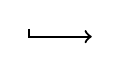
\begin{tikzpicture}
\draw [->, thick] (0.2,0.2) -- (0.2,0.1) -- (1,0.1);
\end{tikzpicture} & \hypertarget{R-3V6.1}{R-3V6.1} & Vincolo

Obbligatorio & La parte destinata agli esaminandi dovrà funzionare si smartphone e tablet iOS dalla versione iOS6 & Capitolato\tabularnewline
\hline
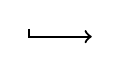
\begin{tikzpicture}
\draw [->, thick] (0.2,0.2) -- (0.2,0.1) -- (1,0.1);
\end{tikzpicture} & \hypertarget{R-3V6.2}{R-3V6.2} & Vincolo

Obbligatorio & La parte destinata agli esaminandi dovrà funzionare su Android dalla versione 4.0 & Capitolato\tabularnewline
\hline
 & \hypertarget{R-3F7}{R-3F7} & Funzionale

Obbligatorio & Il sistema deve gestire questionari & Capitolato

\hyperlink{UC6}{UC6}\tabularnewline
\hline
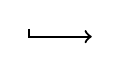
\begin{tikzpicture}
\draw [->, thick] (0.2,0.2) -- (0.2,0.1) -- (1,0.1);
\end{tikzpicture} & \hypertarget{R-3F7.1}{R-3F7.1} & Funzionale

Obbligatorio & L'applicazione deve archiviare questionari in un server, suddivisi per argomento
 & Capitolato\tabularnewline
\hline
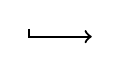
\begin{tikzpicture}
\draw [->, thick] (0.2,0.2) -- (0.2,0.1) -- (1,0.1);
\end{tikzpicture} & \hypertarget{R-3F7.2}{R-3F7.2} & Funzionale

Obbligatorio & L'applicazione deve tradurre da QML a HTML le domande archiviate & Capitolato

\hyperlink{UC13.1}{UC13.1}

\hyperlink{UC5.12}{UC5.12}

\hyperlink{UC5}{UC5}

\hyperlink{UC6}{UC6}\tabularnewline
\hline
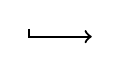
\begin{tikzpicture}
\draw [->, thick] (0.2,0.2) -- (0.2,0.1) -- (1,0.1);
\end{tikzpicture} & \hypertarget{R-3F7.3}{R-3F7.3} & Funzionale

Obbligatorio & L'applicazione deve proporre questionari preconfezionati & Capitolato

\hyperlink{UC6}{UC6}\tabularnewline
\hline
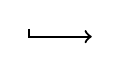
\begin{tikzpicture}
\draw [->, thick] (0.2,0.2) -- (0.2,0.1) -- (1,0.1);
\end{tikzpicture} & \hypertarget{R-3F7.4}{R-3F7.4} & Funzionale

Obbligatorio & L'applicazione deve valutare le risposte fornite dall'utente & Capitolato

\hyperlink{UC13.11}{UC13.11}

\hyperlink{UC13}{UC13}

\hyperlink{UC15}{UC15}\tabularnewline
\hline
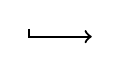
\begin{tikzpicture}
\draw [->, thick] (0.2,0.2) -- (0.2,0.1) -- (1,0.1);
\end{tikzpicture} & \hypertarget{R-3F7.5}{R-3F7.5} & Funzionale

Obbligatorio & Le domande dovranno essere raccolte attraverso uno specifico linguaggio, che chiameremo Quiz Markup Language (QML), studiato per descrivere quiz
 & Capitolato

\hyperlink{UC5.1.2}{UC5.1.2}\tabularnewline
\hline
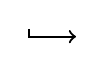
\begin{tikzpicture}
\draw [->, thick] (0.4,0.2) -- (0.4,0.1) -- (1,0.1);
\end{tikzpicture} & \hypertarget{R-3F7.5.1}{R-3F7.5.1} & Funzionale

Obbligatorio & Il QML deve essere un linguaggio semplice con un parsing ad hoc definito dal gruppo. La sintassi per scrivere il testo della domanda deve essere unica, la sintassi per le risposte è dipendente dal tipo di domanda & Capitolato

\hyperlink{UC5.1.2}{UC5.1.2}\tabularnewline
\hline
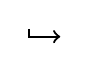
\begin{tikzpicture}
\draw [->, thick] (0.6,0.2) -- (0.6,0.1) -- (1,0.1);
\end{tikzpicture} & \hypertarget{R-2F7.5.1.1}{R-2F7.5.1.1} & Funzionale

Opzionale & Il QML deve permettere l'inserimento di testo in grassetto & \hyperlink{UC5.1.2}{UC5.1.2}\tabularnewline
\hline
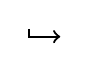
\begin{tikzpicture}
\draw [->, thick] (0.6,0.2) -- (0.6,0.1) -- (1,0.1);
\end{tikzpicture} & \hypertarget{R-3F7.5.1.2}{R-3F7.5.1.2} & Funzionale

Obbligatorio & Il QML deve permettere l'inserimento di immagini & Capitolato

\hyperlink{UC5.1.2}{UC5.1.2}\tabularnewline
\hline
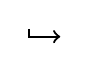
\begin{tikzpicture}
\draw [->, thick] (0.6,0.2) -- (0.6,0.1) -- (1,0.1);
\end{tikzpicture} & \hypertarget{R-2F7.5.1.3}{R-2F7.5.1.3} & Funzionale

Opzionale & Il QML deve permettere l'inserimento di testo in corsivo & \hyperlink{UC5.1.2}{UC5.1.2}\tabularnewline
\hline
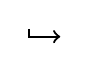
\begin{tikzpicture}
\draw [->, thick] (0.6,0.2) -- (0.6,0.1) -- (1,0.1);
\end{tikzpicture} & \hypertarget{R-2F7.5.1.4}{R-2F7.5.1.4} & Funzionale

Opzionale & Il QML deve permettere l'inserimento di tabelle & \hyperlink{UC5.1.2}{UC5.1.2}\tabularnewline
\hline
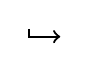
\begin{tikzpicture}
\draw [->, thick] (0.6,0.2) -- (0.6,0.1) -- (1,0.1);
\end{tikzpicture} & \hypertarget{R-2F7.5.1.5}{R-2F7.5.1.5} & Funzionale

Opzionale & Il QML deve permettere di definire un punteggio per ogni risposta & \hyperlink{UC5.1.2}{UC5.1.2}\tabularnewline
\hline
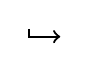
\begin{tikzpicture}
\draw [->, thick] (0.6,0.2) -- (0.6,0.1) -- (1,0.1);
\end{tikzpicture} & \hypertarget{R-3F7.5.1.6}{R-3F7.5.1.6} & Funzionale

Obbligatorio & Il QML deve permettere di definire il tipo di domanda & \hyperlink{UC5.1.2}{UC5.1.2}\tabularnewline
\hline
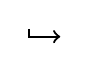
\begin{tikzpicture}
\draw [->, thick] (0.6,0.2) -- (0.6,0.1) -- (1,0.1);
\end{tikzpicture} & \hypertarget{R-2F7.5.1.7}{R-2F7.5.1.7} & Funzionale

Opzionale & Il QML deve permettere l'inserimento di video & \hyperlink{UC5.1.2}{UC5.1.2}

\hyperlink{UC5.1.3}{UC5.1.3}\tabularnewline
\hline
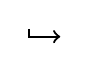
\begin{tikzpicture}
\draw [->, thick] (0.6,0.2) -- (0.6,0.1) -- (1,0.1);
\end{tikzpicture} & \hypertarget{R-2F7.5.1.8}{R-2F7.5.1.8} & Funzionale

Opzionale & Il QML deve permettere l'inserimento di audio & \hyperlink{UC5.1.2}{UC5.1.2}

\hyperlink{UC5.1.3}{UC5.1.3}\tabularnewline
\hline
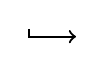
\begin{tikzpicture}
\draw [->, thick] (0.4,0.2) -- (0.4,0.1) -- (1,0.1);
\end{tikzpicture} & \hypertarget{R-2F7.5.2}{R-2F7.5.2} & Funzionale

Opzionale & Il QML può gestire risposte a scelta multipla, a riempimento di parole omesse, ad associazione, a risposta aperta, con testi e immagini & Capitolato

\hyperlink{UC5.10}{UC5.10}

\hyperlink{UC5.11}{UC5.11}

\hyperlink{UC5.1}{UC5.1}

\hyperlink{UC5.7}{UC5.7}

\hyperlink{UC5.9}{UC5.9}\tabularnewline
\hline
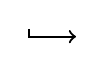
\begin{tikzpicture}
\draw [->, thick] (0.4,0.2) -- (0.4,0.1) -- (1,0.1);
\end{tikzpicture} & \hypertarget{R-3F7.5.3}{R-3F7.5.3} & Funzionale

Obbligatorio & Le domande scritte in QML devono essere editabili dall'utente & Proponente

\hyperlink{UC5.1}{UC5.1}\tabularnewline
\hline
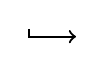
\begin{tikzpicture}
\draw [->, thick] (0.4,0.2) -- (0.4,0.1) -- (1,0.1);
\end{tikzpicture} & \hypertarget{R-2F7.5.4}{R-2F7.5.4} & Funzionale

Opzionale & Le domande possono essere inserite e editabili attraverso interfaccia grafica & Proponente

\hyperlink{UC5.1.3}{UC5.1.3}\tabularnewline
\hline
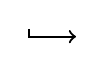
\begin{tikzpicture}
\draw [->, thick] (0.4,0.2) -- (0.4,0.1) -- (1,0.1);
\end{tikzpicture} & \hypertarget{R-3F7.5.5}{R-3F7.5.5} & Funzionale

Obbligatorio & Il QML deve gestire risposte vero/falso e risposte a scelta multipla con testi e immagini & Capitolato

\hyperlink{UC5.1}{UC5.1}

\hyperlink{UC5.6}{UC5.6}

\hyperlink{UC5.8}{UC5.8}\tabularnewline
\hline
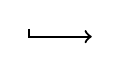
\begin{tikzpicture}
\draw [->, thick] (0.2,0.2) -- (0.2,0.1) -- (1,0.1);
\end{tikzpicture} & \hypertarget{R-2F7.6}{R-2F7.6} & Funzionale

Opzionale & Il sistema deve gestire sia questionari pubblici che privati attraverso la creazione di classi la cui iscrizione è protetta da password & Proponente

\hyperlink{UC14}{UC14}

\hyperlink{UC7.1}{UC7.1}\tabularnewline
\hline
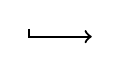
\begin{tikzpicture}
\draw [->, thick] (0.2,0.2) -- (0.2,0.1) -- (1,0.1);
\end{tikzpicture} & \hypertarget{R-3F7.7}{R-3F7.7} & Funzionale

Obbligatorio & I docenti costruiranno questionari scegliendo tra le domande archiviate nel server & Capitolato

\hyperlink{UC6.1}{UC6.1}

\hyperlink{UC6}{UC6}\tabularnewline
\hline
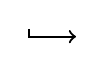
\begin{tikzpicture}
\draw [->, thick] (0.4,0.2) -- (0.4,0.1) -- (1,0.1);
\end{tikzpicture} & \hypertarget{R-3F7.7.1}{R-3F7.7.1} & Funzionale

Obbligatorio & Il sistema deve segnalare un errore nel caso un questionario creato non contenga domande & \hyperlink{UC6.1}{UC6.1}

\hyperlink{UC6.4}{UC6.4}

\hyperlink{UC6}{UC6}\tabularnewline
\hline
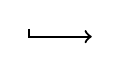
\begin{tikzpicture}
\draw [->, thick] (0.2,0.2) -- (0.2,0.1) -- (1,0.1);
\end{tikzpicture} & \hypertarget{R-2F7.8}{R-2F7.8} & Funzionale

Opzionale & Il sistema deve offrire la possibilità di creare dinamicamente i questionari & Capitolato\tabularnewline
\hline
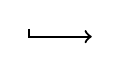
\begin{tikzpicture}
\draw [->, thick] (0.2,0.2) -- (0.2,0.1) -- (1,0.1);
\end{tikzpicture} & \hypertarget{R-2F7.9}{R-2F7.9} & Funzionale

Opzionale & L'applicazione deve essere predisposta ad un sistema di feedback per i questionari & Capitolato

\hyperlink{UC13.10}{UC13.10}\tabularnewline
\hline
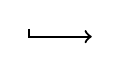
\begin{tikzpicture}
\draw [->, thick] (0.2,0.2) -- (0.2,0.1) -- (1,0.1);
\end{tikzpicture} & \hypertarget{R-2F7.10}{R-2F7.10} & Funzionale

Opzionale & Il sistema deve permettere la raccolta dei dati relativi a questionari svolti & Capitolato

\hyperlink{UC15}{UC15}\tabularnewline
\hline
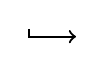
\begin{tikzpicture}
\draw [->, thick] (0.4,0.2) -- (0.4,0.1) -- (1,0.1);
\end{tikzpicture} & \hypertarget{R-2F7.10.1}{R-2F7.10.1} & Funzionale

Opzionale & Il sistema deve permettere la rivisitazione del test svolto e dei risultati ottenuti & Capitolato

\hyperlink{UC15}{UC15}\tabularnewline
\hline
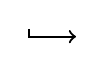
\begin{tikzpicture}
\draw [->, thick] (0.4,0.2) -- (0.4,0.1) -- (1,0.1);
\end{tikzpicture} & \hypertarget{R-2F7.10.2}{R-2F7.10.2} & Funzionale

Opzionale & Il sistema deve offrire la possibilità di analizzare i dati raccolti dai test effettuati & Capitolato

\hyperlink{UC15.2}{UC15.2}

\hyperlink{UC15}{UC15}\tabularnewline
\hline
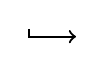
\begin{tikzpicture}
\draw [->, thick] (0.4,0.2) -- (0.4,0.1) -- (1,0.1);
\end{tikzpicture} & \hypertarget{R-2F7.10.3}{R-2F7.10.3} & Funzionale

Opzionale & Il sistema deve offrire la possibilità di visualizzazione sotto forma di grafico delle statistiche dei dati raccolti & Capitolato

\hyperlink{UC15.3}{UC15.3}

\hyperlink{UC15}{UC15}\tabularnewline
\hline
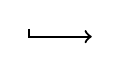
\begin{tikzpicture}
\draw [->, thick] (0.2,0.2) -- (0.2,0.1) -- (1,0.1);
\end{tikzpicture} & \hypertarget{R-3F7.11}{R-3F7.11} & Funzionale

Obbligatorio & Il sistema deve prevedere la gestione di domande & \hyperlink{UC5}{UC5}

\hyperlink{UC6.1.1}{UC6.1.1}

\hyperlink{UC6.1.2}{UC6.1.2}

\hyperlink{UC6}{UC6}\tabularnewline
\hline
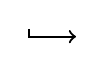
\begin{tikzpicture}
\draw [->, thick] (0.4,0.2) -- (0.4,0.1) -- (1,0.1);
\end{tikzpicture} & \hypertarget{R-3F7.11.1}{R-3F7.11.1} & Funzionale

Obbligatorio & Il sistema deve consentire ad un docente di inserire una nuova domanda & \hyperlink{UC5.1}{UC5.1}

\hyperlink{UC5}{UC5}\tabularnewline
\hline
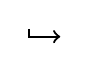
\begin{tikzpicture}
\draw [->, thick] (0.6,0.2) -- (0.6,0.1) -- (1,0.1);
\end{tikzpicture} & \hypertarget{R-3F7.11.1.1}{R-3F7.11.1.1} & Funzionale

Obbligatorio & Un docente deve poter selezionare gli argomenti di una domanda & \hyperlink{UC5.1.1}{UC5.1.1}

\hyperlink{UC5.1}{UC5.1}

\hyperlink{UC5}{UC5}\tabularnewline
\hline
\begin{tikzpicture}
\draw [->, thick] (0.8,0.2) -- (0.8,0.1) -- (1,0.1);
\end{tikzpicture} & \hypertarget{R-3F7.11.1.1.1}{R-3F7.11.1.1.1} & Funzionale

Obbligatorio & Il sistema deve segnalare un errore nel caso non venga selezionato alcun argomento per una nuova domanda & \hyperlink{UC5.1.1}{UC5.1.1}

\hyperlink{UC5.5}{UC5.5}

\hyperlink{UC5}{UC5}

\hyperlink{UC6.1.1}{UC6.1.1}\tabularnewline
\hline
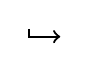
\begin{tikzpicture}
\draw [->, thick] (0.6,0.2) -- (0.6,0.1) -- (1,0.1);
\end{tikzpicture} & \hypertarget{R-3F7.11.1.2}{R-3F7.11.1.2} & Funzionale

Obbligatorio & Un docente deve comporre la domanda da inserire in QML & \hyperlink{UC5.1.2}{UC5.1.2}

\hyperlink{UC5}{UC5}

\hyperlink{UC6.1.1}{UC6.1.1}\tabularnewline
\hline
\begin{tikzpicture}
\draw [->, thick] (0.8,0.2) -- (0.8,0.1) -- (1,0.1);
\end{tikzpicture} & \hypertarget{R-3F7.11.1.2.1}{R-3F7.11.1.2.1} & Funzionale

Obbligatorio & Il sistema deve segnalare un errore nel caso di inserimento QML non valido & \hyperlink{UC5.1.2}{UC5.1.2}

\hyperlink{UC5.4}{UC5.4}

\hyperlink{UC5}{UC5}

\hyperlink{UC6.1.1}{UC6.1.1}\tabularnewline
\hline
\begin{tikzpicture}
\draw [->, thick] (0.8,0.2) -- (0.8,0.1) -- (1,0.1);
\end{tikzpicture} & \hypertarget{R-3F7.11.1.2.2}{R-3F7.11.1.2.2} & Funzionale

Obbligatorio & Il docente deve poter inserire domande di tipo vero/falso & \hyperlink{UC5.1}{UC5.1}

\hyperlink{UC5.6}{UC5.6}\tabularnewline
\hline
\begin{tikzpicture}
\draw [->, thick] (0.8,0.2) -- (0.8,0.1) -- (1,0.1);
\end{tikzpicture} & \hypertarget{R-3F7.11.1.2.3}{R-3F7.11.1.2.3} & Funzionale

Obbligatorio & Il docente deve poter inserire domande a scelta multipla & \hyperlink{UC5.1}{UC5.1}

\hyperlink{UC5.7}{UC5.7}\tabularnewline
\hline
\begin{tikzpicture}
\draw [->, thick] (0.8,0.2) -- (0.8,0.1) -- (1,0.1);
\end{tikzpicture} & \hypertarget{R-1F7.11.1.2.4}{R-1F7.11.1.2.4} & Funzionale

Desiderabile & Il docente deve poter inserire domande a risposta multipla & \hyperlink{UC5.1}{UC5.1}

\hyperlink{UC5.8}{UC5.8}\tabularnewline
\hline
\begin{tikzpicture}
\draw [->, thick] (0.8,0.2) -- (0.8,0.1) -- (1,0.1);
\end{tikzpicture} & \hypertarget{R-1F7.11.1.2.5}{R-1F7.11.1.2.5} & Funzionale

Desiderabile & Il docente deve poter inserire domande di tipo testo con parole omesse & \hyperlink{UC5.1}{UC5.1}

\hyperlink{UC5.9}{UC5.9}\tabularnewline
\hline
\begin{tikzpicture}
\draw [->, thick] (0.8,0.2) -- (0.8,0.1) -- (1,0.1);
\end{tikzpicture} & \hypertarget{R-1F7.11.1.2.6}{R-1F7.11.1.2.6} & Funzionale

Desiderabile & Il docente deve poter inserire domande con associazione di parole & \hyperlink{UC5.10}{UC5.10}

\hyperlink{UC5.1}{UC5.1}\tabularnewline
\hline
\begin{tikzpicture}
\draw [->, thick] (0.8,0.2) -- (0.8,0.1) -- (1,0.1);
\end{tikzpicture} & \hypertarget{R-2F7.11.1.2.7}{R-2F7.11.1.2.7} & Funzionale

Opzionale & Il docente deve poter inserire domande a risposta aperta & \hyperlink{UC5.11}{UC5.11}

\hyperlink{UC5.1}{UC5.1}\tabularnewline
\hline
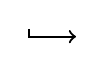
\begin{tikzpicture}
\draw [->, thick] (0.4,0.2) -- (0.4,0.1) -- (1,0.1);
\end{tikzpicture} & \hypertarget{R-3F7.11.2}{R-3F7.11.2} & Funzionale

Obbligatorio & Il sistema deve consentire ad un docente di modificare una domanda & \hyperlink{UC5.2}{UC5.2}

\hyperlink{UC5}{UC5}\tabularnewline
\hline
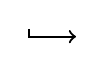
\begin{tikzpicture}
\draw [->, thick] (0.4,0.2) -- (0.4,0.1) -- (1,0.1);
\end{tikzpicture} & \hypertarget{R-3F7.11.3}{R-3F7.11.3} & Funzionale

Obbligatorio & Il sistema deve consentire ad un docente di eliminare una propria domanda presente nel sistema & \hyperlink{UC5.3}{UC5.3}

\hyperlink{UC5}{UC5}\tabularnewline
\hline
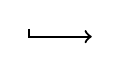
\begin{tikzpicture}
\draw [->, thick] (0.2,0.2) -- (0.2,0.1) -- (1,0.1);
\end{tikzpicture} & \hypertarget{R-3F7.12}{R-3F7.12} & Funzionale

Obbligatorio & il sistema deve dare la possibilità al docente di modificare il proprio questionario & \hyperlink{UC6.2}{UC6.2}

\hyperlink{UC6}{UC6}\tabularnewline
\hline
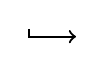
\begin{tikzpicture}
\draw [->, thick] (0.4,0.2) -- (0.4,0.1) -- (1,0.1);
\end{tikzpicture} & \hypertarget{R-3F7.12.1}{R-3F7.12.1} & Funzionale

Obbligatorio & Il sistema deve dare la possibilità di ricercare un questionario & \hyperlink{UC16}{UC16}\tabularnewline
\hline
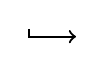
\begin{tikzpicture}
\draw [->, thick] (0.4,0.2) -- (0.4,0.1) -- (1,0.1);
\end{tikzpicture} & \hypertarget{R-3F7.12.2}{R-3F7.12.2} & Funzionale

Obbligatorio & Il sistema deve dare la possibile al docente di aggiungere al questionario già fatto una domanda. & \hyperlink{UC6.2.1}{UC6.2.1}

\hyperlink{UC6}{UC6}\tabularnewline
\hline
\begin{tikzpicture}
\draw [->, thick] (0.4,0.2) -- (0.4,0.1) -- (1,0.1);
\end{tikzpicture} & \hypertarget{R-3F7.12.3}{R-3F7.12.3} & Funzionale

Obbligatorio & Il sistema deve dare la possibilità al docente di togliere domande precedentemente aggiunte al questionario & \hyperlink{UC6.2.2}{UC6.2.2}

\hyperlink{UC6}{UC6}\tabularnewline
\hline
\begin{tikzpicture}
\draw [->, thick] (0.4,0.2) -- (0.4,0.1) -- (1,0.1);
\end{tikzpicture} & \hypertarget{R-3F7.12.4}{R-3F7.12.4} & Funzionale

Obbligatorio & Il sistema deve consentire ad un docente di modificare gli argomenti di un proprio questionario & \hyperlink{UC6.2.3}{UC6.2.3}

\hyperlink{UC6.2}{UC6.2}

\hyperlink{UC6}{UC6}\tabularnewline
\hline
\begin{tikzpicture}
\draw [->, thick] (0.2,0.2) -- (0.2,0.1) -- (1,0.1);
\end{tikzpicture} & \hypertarget{R-3F7.13}{R-3F7.13} & Funzionale

Obbligatorio & Il sistema deve dare la possibilità al docente di eliminare il proprio questionario & \hyperlink{UC6.3}{UC6.3}

\hyperlink{UC6}{UC6}\tabularnewline
\hline
 & \hypertarget{R-3F8}{R-3F8} & Funzionale

Obbligatorio & L'utente attraverso una specifica interfaccia potrà rispondere alle domande & Capitolato

\hyperlink{UC13.1}{UC13.1}\tabularnewline
\hline
 & \hypertarget{R-3F9}{R-3F9} & Funzionale

Obbligatorio & Il sistema deve avere almeno 3 tipi di utenti: amministratore, docente e studente & Capitolato\tabularnewline
\hline
 & \hypertarget{R-3F10}{R-3F10} & Funzionale

Obbligatorio & Il sistema deve gestire la registrazione di un utente & \hyperlink{UC2}{UC2}\tabularnewline
\hline
\begin{tikzpicture}
\draw [->, thick] (0.2,0.2) -- (0.2,0.1) -- (1,0.1);
\end{tikzpicture} & \hypertarget{R-3F10.1}{R-3F10.1} & Funzionale

Obbligatorio & Il sistema deve già possedere un proprietario all'installazione del sistema & Interno\tabularnewline
\hline
\begin{tikzpicture}
\draw [->, thick] (0.2,0.2) -- (0.2,0.1) -- (1,0.1);
\end{tikzpicture} & \hypertarget{R-3F10.2}{R-3F10.2} & Funzionale

Obbligatorio & La registrazione di un utente richiede l’inserimento di uno username, password e nome completo  & \hyperlink{UC2.1}{UC2.1}

\hyperlink{UC2.2}{UC2.2}

\hyperlink{UC2.3}{UC2.3}\tabularnewline
\hline
\begin{tikzpicture}
\draw [->, thick] (0.4,0.2) -- (0.4,0.1) -- (1,0.1);
\end{tikzpicture} & \hypertarget{R-3F10.2.1}{R-3F10.2.1} & Funzionale

Obbligatorio & Il sistema deve segnalare un errore nel caso non vengano inseriti tutti i campi necessari per la registrazione & \hyperlink{UC2.4}{UC2.4}

\hyperlink{UC2.5}{UC2.5}

\hyperlink{UC2.6}{UC2.6}

\hyperlink{UC2.7}{UC2.7}\tabularnewline
\hline
\begin{tikzpicture}
\draw [->, thick] (0.4,0.2) -- (0.4,0.1) -- (1,0.1);
\end{tikzpicture} & \hypertarget{R-3F10.2.2}{R-3F10.2.2} & Funzionale

Obbligatorio & La registrazione di uno utente deve richiedere l'inserimento delle informazioni personali & \hyperlink{UC2.1}{UC2.1}\tabularnewline
\hline
\begin{tikzpicture}
\draw [->, thick] (0.2,0.2) -- (0.2,0.1) -- (1,0.1);
\end{tikzpicture} & \hypertarget{R-3F10.3}{R-3F10.3} & Funzionale

Obbligatorio & Il sistema deve permettere la visualizzazione di un messaggio di errore se l'username dell' utente è già presente nel sistema & \hyperlink{UC2.7}{UC2.7}\tabularnewline
\hline
\begin{tikzpicture}
\draw [->, thick] (0.2,0.2) -- (0.2,0.1) -- (1,0.1);
\end{tikzpicture} & \hypertarget{R-3F10.4}{R-3F10.4} & Funzionale

Obbligatorio & Il sistema deve permettere la visualizzazione di un messaggio di errore se la password dell'utente è troppo corta & \hyperlink{UC2.6}{UC2.6}\tabularnewline
\hline
\begin{tikzpicture}
\draw [->, thick] (0.2,0.2) -- (0.2,0.1) -- (1,0.1);
\end{tikzpicture} & \hypertarget{R-3F10.5}{R-3F10.5} & Funzionale

Obbligatorio & Il sistema deve segnalare un errore se viene inserito un username già utilizzato & \hyperlink{UC2.7}{UC2.7}\tabularnewline
\hline
 & \hypertarget{R-3V11}{R-3V11} & Vincolo

Obbligatorio & Il database server side deve essere MongoDB & Capitolato

Interno\tabularnewline
\hline
 & \hypertarget{R-3F12}{R-3F12} & Funzionale

Obbligatorio & Il sistema deve gestire le azioni di amministratore & \hyperlink{UC30}{UC30}\tabularnewline
\hline
\begin{tikzpicture}
\draw [->, thick] (0.2,0.2) -- (0.2,0.1) -- (1,0.1);
\end{tikzpicture} & \hypertarget{R-3F12.1}{R-3F12.1} & Funzionale

Obbligatorio & L'amministratore deve poter cambiare il ruolo di un utente con grado inferiore al proprio in un ruolo con grado inferiore al proprio & \hyperlink{UC30.1}{UC30.1}

\hyperlink{UC30}{UC30}\tabularnewline
\hline
\begin{tikzpicture}
\draw [->, thick] (0.2,0.2) -- (0.2,0.1) -- (1,0.1);
\end{tikzpicture} & \hypertarget{R-3F12.2}{R-3F12.2} & Funzionale

Obbligatorio & Il sistema deve dare la possibilità ad un amministratore o proprietario di eliminare un utente di ruolo inferiore al proprio & \hyperlink{UC30.2}{UC30.2}

\hyperlink{UC30}{UC30}\tabularnewline
\hline
 & \hypertarget{R-2F13}{R-2F13} & Funzionale

Opzionale & Il sistema deve prevedere la gestione di classi da parte di un docente & \hyperlink{UC7}{UC7}\tabularnewline
\hline
\begin{tikzpicture}
\draw [->, thick] (0.2,0.2) -- (0.2,0.1) -- (1,0.1);
\end{tikzpicture} & \hypertarget{R-2F13.1}{R-2F13.1} & Funzionale

Opzionale & Un docente deve avere la possibilità di creare una nuova classe & \hyperlink{UC7.1}{UC7.1}

\hyperlink{UC7}{UC7}\tabularnewline
\hline
\begin{tikzpicture}
\draw [->, thick] (0.4,0.2) -- (0.4,0.1) -- (1,0.1);
\end{tikzpicture} & \hypertarget{R-2F13.1.1}{R-2F13.1.1} & Funzionale

Opzionale & Un docente deve poter specificare il nome della nuova classe & \hyperlink{UC7.1.1}{UC7.1.1}

\hyperlink{UC7.1}{UC7.1}

\hyperlink{UC7}{UC7}\tabularnewline
\hline
\begin{tikzpicture}
\draw [->, thick] (0.6,0.2) -- (0.6,0.1) -- (1,0.1);
\end{tikzpicture} & \hypertarget{R-2F13.1.1.1}{R-2F13.1.1.1} & Funzionale

Opzionale & Nel caso il nome della classe sia già presente il sistema deve segnalare un errore & \hyperlink{UC7.1.1}{UC7.1.1}

\hyperlink{UC7.1}{UC7.1}

\hyperlink{UC7.4}{UC7.4}

\hyperlink{UC7}{UC7}\tabularnewline
\hline
\begin{tikzpicture}
\draw [->, thick] (0.4,0.2) -- (0.4,0.1) -- (1,0.1);
\end{tikzpicture} & \hypertarget{R-2F13.1.2}{R-2F13.1.2} & Funzionale

Opzionale & Un docente deve poter specificare gli argomenti di una nuova classe & \hyperlink{UC7.1.2}{UC7.1.2}

\hyperlink{UC7.1}{UC7.1}

\hyperlink{UC7}{UC7}\tabularnewline
\hline
\begin{tikzpicture}
\draw [->, thick] (0.4,0.2) -- (0.4,0.1) -- (1,0.1);
\end{tikzpicture} & \hypertarget{R-2F13.1.3}{R-2F13.1.3} & Funzionale

Opzionale & Un docente deve poter specificare la password relativa ad una nuova classe & \hyperlink{UC7.1.3}{UC7.1.3}

\hyperlink{UC7.1}{UC7.1}

\hyperlink{UC7}{UC7}\tabularnewline
\hline
\begin{tikzpicture}
\draw [->, thick] (0.2,0.2) -- (0.2,0.1) -- (1,0.1);
\end{tikzpicture} & \hypertarget{R-2F13.2}{R-2F13.2} & Funzionale

Opzionale & Un docente deve avere la possibilità di eliminare una classe esistente & \hyperlink{UC7.3}{UC7.3}

\hyperlink{UC7}{UC7}\tabularnewline
\hline
\begin{tikzpicture}
\draw [->, thick] (0.2,0.2) -- (0.2,0.1) -- (1,0.1);
\end{tikzpicture} & \hypertarget{R-2F13.3}{R-2F13.3} & Funzionale

Opzionale & Un docente deve poter modificare una classe & \hyperlink{UC7.2}{UC7.2}

\hyperlink{UC7}{UC7}\tabularnewline
\hline
\begin{tikzpicture}
\draw [->, thick] (0.4,0.2) -- (0.4,0.1) -- (1,0.1);
\end{tikzpicture} & \hypertarget{R-2F13.3.1}{R-2F13.3.1} & Funzionale

Opzionale & Un docente deve poter modificare il nome di una propria classe esistente & \hyperlink{UC7.1.1}{UC7.1.1}

\hyperlink{UC7.2}{UC7.2}

\hyperlink{UC7}{UC7}\tabularnewline
\hline
\begin{tikzpicture}
\draw [->, thick] (0.4,0.2) -- (0.4,0.1) -- (1,0.1);
\end{tikzpicture} & \hypertarget{R-2F13.3.2}{R-2F13.3.2} & Funzionale

Opzionale & Un docente deve poter modificare gli argomenti di una sua classe esistente & \hyperlink{UC7.1.2}{UC7.1.2}

\hyperlink{UC7.2}{UC7.2}

\hyperlink{UC7}{UC7}\tabularnewline
\hline
\begin{tikzpicture}
\draw [->, thick] (0.4,0.2) -- (0.4,0.1) -- (1,0.1);
\end{tikzpicture} & \hypertarget{R-2F13.3.3}{R-2F13.3.3} & Funzionale

Opzionale & Un docente deve poter modificare la password di una delle proprie classi & \hyperlink{UC7.1.3}{UC7.1.3}

\hyperlink{UC7.2}{UC7.2}

\hyperlink{UC7}{UC7}\tabularnewline
\hline
 & \hypertarget{R-3F14}{R-3F14} & Funzionale

Obbligatorio & Il sistema deve consentire ad un utente di gestire i propri dati memorizzati nel sistema & \hyperlink{UC3}{UC3}\tabularnewline
\hline
\begin{tikzpicture}
\draw [->, thick] (0.2,0.2) -- (0.2,0.1) -- (1,0.1);
\end{tikzpicture} & \hypertarget{R-3F14.1}{R-3F14.1} & Funzionale

Obbligatorio & Il sistema deve consentire ad un utente di modificare la propria username & \hyperlink{UC3.2}{UC3.2}

\hyperlink{UC3}{UC3}\tabularnewline
\hline
\begin{tikzpicture}
\draw [->, thick] (0.4,0.2) -- (0.4,0.1) -- (1,0.1);
\end{tikzpicture} & \hypertarget{R-3F14.1.1}{R-3F14.1.1} & Funzionale

Obbligatorio & Il sistema deve gestire eventuali errori di inserimento username & \hyperlink{UC3.2}{UC3.2}

\hyperlink{UC3.4}{UC3.4}

\hyperlink{UC3.6}{UC3.6}

\hyperlink{UC3}{UC3}\tabularnewline
\hline
\begin{tikzpicture}
\draw [->, thick] (0.4,0.2) -- (0.4,0.1) -- (1,0.1);
\end{tikzpicture} & \hypertarget{R-3F14.1.2}{R-3F14.1.2} & Funzionale

Obbligatorio & Il sistema deve segnalare un errore in caso di inserimento di username già presente nel sistema & \hyperlink{UC3.6}{UC3.6}

\hyperlink{UC3}{UC3}\tabularnewline
\hline
\begin{tikzpicture}
\draw [->, thick] (0.2,0.2) -- (0.2,0.1) -- (1,0.1);
\end{tikzpicture} & \hypertarget{R-3F14.2}{R-3F14.2} & Funzionale

Obbligatorio & Il sistema deve consentire ad un utente di modificare la propria password di accesso al sistema & \hyperlink{UC3.3}{UC3.3}

\hyperlink{UC3}{UC3}\tabularnewline
\hline
\begin{tikzpicture}
\draw [->, thick] (0.4,0.2) -- (0.4,0.1) -- (1,0.1);
\end{tikzpicture} & \hypertarget{R-3F14.2.1}{R-3F14.2.1} & Funzionale

Obbligatorio & Il sistema deve richiedere l'inserimento della vecchia password all'utente per consentire la modifica della password & \hyperlink{UC3.3.1}{UC3.3.1}

\hyperlink{UC3.3}{UC3.3}

\hyperlink{UC3}{UC3}\tabularnewline
\hline
\begin{tikzpicture}
\draw [->, thick] (0.6,0.2) -- (0.6,0.1) -- (1,0.1);
\end{tikzpicture} & \hypertarget{R-3F14.2.1.1}{R-3F14.2.1.1} & Funzionale

Obbligatorio & Il sistema deve segnalare l'inserimento di una password scorretta & \hyperlink{UC3.3.2}{UC3.3.2}

\hyperlink{UC3.7}{UC3.7}

\hyperlink{UC3}{UC3}\tabularnewline
\hline
\begin{tikzpicture}
\draw [->, thick] (0.4,0.2) -- (0.4,0.1) -- (1,0.1);
\end{tikzpicture} & \hypertarget{R-3F14.2.2}{R-3F14.2.2} & Funzionale

Obbligatorio & Il sistema deve richiedere l'inserimento della nuova password & \hyperlink{UC3.3}{UC3.3}

\hyperlink{UC3}{UC3}\tabularnewline
\hline
\begin{tikzpicture}
\draw [->, thick] (0.6,0.2) -- (0.6,0.1) -- (1,0.1);
\end{tikzpicture} & \hypertarget{R-3F14.2.2.1}{R-3F14.2.2.1} & Funzionale

Obbligatorio & Il sistema deve verificare che la nuova password sia di almeno otto caratteri e segnalarlo in caso contrario & \hyperlink{UC3.3}{UC3.3}

\hyperlink{UC3.7}{UC3.7}

\hyperlink{UC3}{UC3}\tabularnewline
\hline
\begin{tikzpicture}
\draw [->, thick] (0.2,0.2) -- (0.2,0.1) -- (1,0.1);
\end{tikzpicture} & \hypertarget{R-3F14.3}{R-3F14.3} & Funzionale

Obbligatorio & Il sistema deve consentire all'utente di modificare i propri dati personali & \hyperlink{UC3.1}{UC3.1}

\hyperlink{UC3.2}{UC3.2}

\hyperlink{UC3}{UC3}\tabularnewline
\hline
\begin{tikzpicture}
\draw [->, thick] (0.4,0.2) -- (0.4,0.1) -- (1,0.1);
\end{tikzpicture} & \hypertarget{R-3F14.3.1}{R-3F14.3.1} & Funzionale

Obbligatorio & Il sistema deve consentire all'utente la modifica del proprio nome  & 

\hyperlink{UC3.1}{UC3.1}

\hyperlink{UC3}{UC3}\tabularnewline
\hline
\begin{tikzpicture}
\draw [->, thick] (0.4,0.2) -- (0.4,0.1) -- (1,0.1);
\end{tikzpicture} & \hypertarget{R-3F14.3.2}{R-3F14.3.2} & Funzionale

Obbligatorio & Il sistema deve consentire all'utente di modificare il proprio username & \hyperlink{UC3.2}{UC3.2}

\hyperlink{UC3}{UC3}\tabularnewline
\hline
\begin{tikzpicture}
\draw [->, thick] (0.4,0.2) -- (0.4,0.1) -- (1,0.1);
\end{tikzpicture} & \hypertarget{R-3F14.3.3}{R-3F14.3.3} & Funzionale

Obbligatorio & Il sistema deve controllare che il nome completo contenga almeno 2 caratteri e in caso contrario mostrare un errore & \hyperlink{UC3.1}{UC3.1}

\hyperlink{UC3.5}{UC3.5}

\hyperlink{UC3}{UC3}\tabularnewline
\hline
\begin{tikzpicture}
\draw [->, thick] (0.4,0.2) -- (0.4,0.1) -- (1,0.1);
\end{tikzpicture} & \hypertarget{R-3F14.3.4}{R-3F14.3.4} & Funzionale

Obbligatorio & Il sistema deve controllare che l'username contenga almeno 6 caratteri e in caso contrario mostrare un errore & \hyperlink{UC3.2}{UC3.2}

\hyperlink{UC3.4}{UC3.4}

\hyperlink{UC3}{UC3}\tabularnewline
\hline
 & \hypertarget{R-3F15}{R-3F15} & Funzionale

Obbligatorio & Il sistema deve gestire la ricerca di un questionario & \hyperlink{UC16}{UC16}\tabularnewline
\hline
\begin{tikzpicture}
\draw [->, thick] (0.2,0.2) -- (0.2,0.1) -- (1,0.1);
\end{tikzpicture} & \hypertarget{R-3F15.1}{R-3F15.1} & Funzionale

Obbligatorio & Il sistema deve gestire la ricerca di un questionario per titolo & \hyperlink{UC16}{UC16}

\hyperlink{UC17}{UC17}\tabularnewline
\hline
\begin{tikzpicture}
\draw [->, thick] (0.2,0.2) -- (0.2,0.1) -- (1,0.1);
\end{tikzpicture} & \hypertarget{R-2F15.2}{R-2F15.2} & Funzionale

Opzionale & Il sistema deve gestire la ricerca di un questionario per classe & \hyperlink{UC16}{UC16}

\hyperlink{UC18}{UC18}\tabularnewline
\hline
\begin{tikzpicture}
\draw [->, thick] (0.2,0.2) -- (0.2,0.1) -- (1,0.1);
\end{tikzpicture} & \hypertarget{R-3F15.3}{R-3F15.3} & Funzionale

Obbligatorio & Il sistema deve gestire la ricerca di un questionario per docente & \hyperlink{UC16}{UC16}

\hyperlink{UC20}{UC20}\tabularnewline
\hline
\begin{tikzpicture}
\draw [->, thick] (0.2,0.2) -- (0.2,0.1) -- (1,0.1);
\end{tikzpicture} & \hypertarget{R-3F15.4}{R-3F15.4} & Funzionale

Obbligatorio & Il sistema deve gestire la ricerca di un questionario per argomento & \hyperlink{UC16}{UC16}

\hyperlink{UC19}{UC19}\tabularnewline
\hline
\begin{tikzpicture}
\draw [->, thick] (0.2,0.2) -- (0.2,0.1) -- (1,0.1);
\end{tikzpicture} & \hypertarget{R-2F15.5}{R-2F15.5} & Funzionale

Opzionale & Il sistema deve gestire la ricerca di un questionario per difficoltà & \hyperlink{UC16}{UC16}

\hyperlink{UC21}{UC21}\tabularnewline
\hline
 & \hypertarget{R-2F16}{R-2F16} & Funzionale

Opzionale & Il sistema deve consentire l'iscrizione ad una classe da parte di uno studente & \hyperlink{UC14}{UC14}\tabularnewline
\hline
\begin{tikzpicture}
\draw [->, thick] (0.2,0.2) -- (0.2,0.1) -- (1,0.1);
\end{tikzpicture} & \hypertarget{R-2F16.1}{R-2F16.1} & Funzionale

Opzionale & Il sistema deve chiedere l'inserimento della password prima di confermare l'iscrizione ad una classe & \hyperlink{UC14.1}{UC14.1}

\hyperlink{UC14}{UC14}\tabularnewline
\hline
\begin{tikzpicture}
\draw [->, thick] (0.4,0.2) -- (0.4,0.1) -- (1,0.1);
\end{tikzpicture} & \hypertarget{R-2F16.1.1}{R-2F16.1.1} & Funzionale

Opzionale & Il sistema deve verificare la password prima di confermare l'iscrizione dello studente alla classe. & \hyperlink{UC14.2}{UC14.2}

\hyperlink{UC14}{UC14}\tabularnewline
\hline
\begin{tikzpicture}
\draw [->, thick] (0.2,0.2) -- (0.2,0.1) -- (1,0.1);
\end{tikzpicture} & \hypertarget{R-2F16.2}{R-2F16.2} & Funzionale

Opzionale & Il sistema deve consentire di ricercare la classe a cui iscriversi & \hyperlink{UC27}{UC27}

\hyperlink{UC28}{UC28}

\hyperlink{UC29}{UC29}\tabularnewline
\hline
 & \hypertarget{R-3F17}{R-3F17} & Funzionale

Obbligatorio & Il sistema deve dare la possibilità di eseguire un questionario ad uno studente & \hyperlink{UC13}{UC13}\tabularnewline
\hline
\begin{tikzpicture}
\draw [->, thick] (0.2,0.2) -- (0.2,0.1) -- (1,0.1);
\end{tikzpicture} & \hypertarget{R-3F17.1}{R-3F17.1} & Funzionale

Obbligatorio & Il sistema deve dare la possibilità ad uno studente di rispondere ad una domanda & \hyperlink{UC13.1}{UC13.1}

\hyperlink{UC13}{UC13}\tabularnewline
\hline
\begin{tikzpicture}
\draw [->, thick] (0.4,0.2) -- (0.4,0.1) -- (1,0.1);
\end{tikzpicture} & \hypertarget{R-3F17.1.1}{R-3F17.1.1} & Funzionale

Obbligatorio & Il sistema deve dare la possibilità ad uno studente di rispondere ad una domanda di tipo vero/falso & \hyperlink{UC13.1}{UC13.1}

\hyperlink{UC13.4}{UC13.4}\tabularnewline
\hline
\begin{tikzpicture}
\draw [->, thick] (0.4,0.2) -- (0.4,0.1) -- (1,0.1);
\end{tikzpicture} & \hypertarget{R-3F17.1.2}{R-3F17.1.2} & Funzionale

Obbligatorio & Il sistema deve dare la possibilità ad uno studente di rispondere ad una domanda a scelta multipla & \hyperlink{UC13.1}{UC13.1}

\hyperlink{UC13.5}{UC13.5}\tabularnewline
\hline
\begin{tikzpicture}
\draw [->, thick] (0.4,0.2) -- (0.4,0.1) -- (1,0.1);
\end{tikzpicture} & \hypertarget{R-1F17.1.3}{R-1F17.1.3} & Funzionale

Desiderabile & Il sistema deve dare la possibilità ad uno studente di rispondere ad una domanda a risposta multipla ovvero una domanda a scelta multipla  con più risposte giuste & \hyperlink{UC13.1}{UC13.1}

\hyperlink{UC13.6}{UC13.6}\tabularnewline
\hline
\begin{tikzpicture}
\draw [->, thick] (0.4,0.2) -- (0.4,0.1) -- (1,0.1);
\end{tikzpicture} & \hypertarget{R-1F17.1.4}{R-1F17.1.4} & Funzionale

Desiderabile & Il sistema deve dare la possibilità ad uno studente di rispondere ad una domanda di tipo testo con parole omesse & \hyperlink{UC13.1}{UC13.1}

\hyperlink{UC13.7}{UC13.7}\tabularnewline
\hline
\begin{tikzpicture}
\draw [->, thick] (0.4,0.2) -- (0.4,0.1) -- (1,0.1);
\end{tikzpicture} & \hypertarget{R-1F17.1.5}{R-1F17.1.5} & Funzionale

Desiderabile & Il sistema deve dare la possibilità ad uno studente di rispondere ad una domanda con associazione di parole & \hyperlink{UC13.1}{UC13.1}

\hyperlink{UC13.8}{UC13.8}\tabularnewline
\hline
\begin{tikzpicture}
\draw [->, thick] (0.4,0.2) -- (0.4,0.1) -- (1,0.1);
\end{tikzpicture} & \hypertarget{R-2F17.1.6}{R-2F17.1.6} & Funzionale

Opzionale & Il sistema deve dare la possibilità ad uno studente di rispondere ad una domanda a risposta aperta & \hyperlink{UC13.1}{UC13.1}

\hyperlink{UC13.9}{UC13.9}\tabularnewline
\hline
\begin{tikzpicture}
\draw [->, thick] (0.2,0.2) -- (0.2,0.1) -- (1,0.1);
\end{tikzpicture} & \hypertarget{R-3F17.2}{R-3F17.2} & Funzionale

Obbligatorio & Il sistema deve richiedere allo studente la conferma alla fine della compilazione di un questionario, perché questo sia considerato eseguito & \hyperlink{UC13.3}{UC13.3}

\hyperlink{UC13}{UC13}\tabularnewline
\hline
\begin{tikzpicture}
\draw [->, thick] (0.4,0.2) -- (0.4,0.1) -- (1,0.1);
\end{tikzpicture} & \hypertarget{R-3F17.2.1}{R-3F17.2.1} & Funzionale

Obbligatorio & Il sistema deve segnalare un errore nel caso una domanda del questionario non sia stata compilata & \hyperlink{UC13.2}{UC13.2}

\hyperlink{UC13.3}{UC13.3}

\hyperlink{UC13}{UC13}\tabularnewline
\hline
\begin{tikzpicture}
\draw [->, thick] (0.2,0.2) -- (0.2,0.1) -- (1,0.1);
\end{tikzpicture} & \hypertarget{R-3F17.3}{R-3F17.3} & Funzionale

Obbligatorio & Il sistema deve dare la possibilità ad uno studente di andare alla domanda successiva durante l'esecuzione del questionario & \hyperlink{UC13}{UC13}\tabularnewline
\hline
\begin{tikzpicture}
\draw [->, thick] (0.2,0.2) -- (0.2,0.1) -- (1,0.1);
\end{tikzpicture} & \hypertarget{R-3F17.4}{R-3F17.4} & Funzionale

Obbligatorio & Il sistema deve dare la possibilità ad uno studente di andare alla domanda precedente durante l'esecuzione del questionario & \hyperlink{UC13}{UC13}\tabularnewline
\hline
 & \hypertarget{R-3F18}{R-3F18} & Funzionale

Obbligatorio & Il sistema deve consentire all'utente autenticato di effettuare il logout & \hyperlink{UC4}{UC4}\tabularnewline
\hline
 & \hypertarget{R-3F19}{R-3F19} & Funzionale

Obbligatorio & Il sistema deve gestire le operazioni che può fare il proprietario del sistema & \hyperlink{UC30}{UC30}\tabularnewline
\hline
\begin{tikzpicture}
\draw [->, thick] (0.2,0.2) -- (0.2,0.1) -- (1,0.1);
\end{tikzpicture} & \hypertarget{R-3F19.1}{R-3F19.1} & Funzionale

Obbligatorio & Il sistema deve assicurare l'esistenza di un unico utente proprietario & Interno\tabularnewline
\hline
\begin{tikzpicture}
\draw [->, thick] (0.2,0.2) -- (0.2,0.1) -- (1,0.1);
\end{tikzpicture} & \hypertarget{R-3F19.2}{R-3F19.2} & Funzionale

Obbligatorio & Il sistema deve consentire solo all'utente proprietario di promuovere un utente al ruolo di amministratore & \hyperlink{UC30.1}{UC30.1}

\hyperlink{UC30}{UC30}\tabularnewline
\hline
\begin{tikzpicture}
\draw [->, thick] (0.2,0.2) -- (0.2,0.1) -- (1,0.1);
\end{tikzpicture} & \hypertarget{R-3F19.3}{R-3F19.3} & Funzionale

Obbligatorio & Il sistema deve consentire solo all'utente proprietario di eliminare un amministratore & \hyperlink{UC30.2}{UC30.2}

\hyperlink{UC30}{UC30}\tabularnewline
\hline
 & \hypertarget{R-3F20}{R-3F20} & Funzionale

Obbligatorio & Il sistema deve consentire ad un docente, amministratore o proprietario di ricercare una domanda presente nel sistema & \hyperlink{UC22}{UC22}\tabularnewline
\hline
\begin{tikzpicture}
\draw [->, thick] (0.2,0.2) -- (0.2,0.1) -- (1,0.1);
\end{tikzpicture} & \hypertarget{R-3F20.1}{R-3F20.1} & Funzionale

Obbligatorio & Il sistema deve consentire a un docente, amministratore o proprietario di ricercare una domanda per argomento & \hyperlink{UC22}{UC22}

\hyperlink{UC24}{UC24}\tabularnewline
\hline
\begin{tikzpicture}
\draw [->, thick] (0.2,0.2) -- (0.2,0.1) -- (1,0.1);
\end{tikzpicture} & \hypertarget{R-3F20.2}{R-3F20.2} & Funzionale

Obbligatorio & Il sistema deve consentire a un docente, amministratore o proprietario di ricercare una domanda per docente & \hyperlink{UC22}{UC22}

\hyperlink{UC26}{UC26}\tabularnewline
\hline
\begin{tikzpicture}
\draw [->, thick] (0.2,0.2) -- (0.2,0.1) -- (1,0.1);
\end{tikzpicture} & \hypertarget{R-2F20.3}{R-2F20.3} & Funzionale

Opzionale & Il sistema deve consentire a un docente, amministratore o proprietario di ricercare una domanda per difficoltà & \hyperlink{UC22}{UC22}

\hyperlink{UC25}{UC25}\tabularnewline
\hline
\begin{tikzpicture}
\draw [->, thick] (0.2,0.2) -- (0.2,0.1) -- (1,0.1);
\end{tikzpicture} & \hypertarget{R-3F20.4}{R-3F20.4} & Funzionale

Obbligatorio & Il sistema deve consentire a un docente, amministratore o proprietario di ricercare una domanda per keywords & \hyperlink{UC22}{UC22}

\hyperlink{UC23}{UC23}\tabularnewline
\hline
 & \hypertarget{R-2F21}{R-2F21} & Funzionale

Opzionale & Il sistema deve fornire la possibilità ad uno studente  di cercare una classe & \hyperlink{UC27}{UC27}\tabularnewline
\hline
\begin{tikzpicture}
\draw [->, thick] (0.2,0.2) -- (0.2,0.1) -- (1,0.1);
\end{tikzpicture} & \hypertarget{R-2F21.1}{R-2F21.1} & Funzionale

Opzionale & Il sistema deve fornire la possibilità ad uno studente  di cercare una classe per argomento & \hyperlink{UC27}{UC27}

\hyperlink{UC29}{UC29}\tabularnewline
\hline
\begin{tikzpicture}
\draw [->, thick] (0.2,0.2) -- (0.2,0.1) -- (1,0.1);
\end{tikzpicture} & \hypertarget{R-2F21.2}{R-2F21.2} & Funzionale

Opzionale & Il sistema deve fornire la possibilità ad uno studente  di cercare una classe per docente & \hyperlink{UC27}{UC27}

\hyperlink{UC28}{UC28}\tabularnewline
\hline
 & \hypertarget{R-2F22}{R-2F22} & Funzionale

Opzionale & Il sistema deve dare la possibilità di recupero password ad un utente non autenticato inviando una mail con la nuova password
 & \hyperlink{UC35}{UC35}\tabularnewline
\hline
\begin{tikzpicture}
\draw [->, thick] (0.2,0.2) -- (0.2,0.1) -- (1,0.1);
\end{tikzpicture} & \hypertarget{R-2F22.1}{R-2F22.1} & Funzionale

Opzionale & Il sistema deve dare la possibilità di inserire  mail per recupero password ad un utente non autenticato & \hyperlink{UC35}{UC35}\tabularnewline
\hline
\begin{tikzpicture}
\draw [->, thick] (0.2,0.2) -- (0.2,0.1) -- (1,0.1);
\end{tikzpicture} & \hypertarget{R-2F22.2}{R-2F22.2} & Funzionale

Opzionale & Il sistema deve segnalare ad un utente non autenticato che l'email inserito per recupero password non è presente nel sistema & \hyperlink{UC35.1}{UC35.1}

\hyperlink{UC35}{UC35}\tabularnewline
\hline
 & \hypertarget{R-3F23}{R-3F23} & Funzionale

Obbligatorio & Il sistema deve permettere ad un docente di gestire gli argomenti & \hyperlink{UC8}{UC8}\tabularnewline
\hline
\begin{tikzpicture}
\draw [->, thick] (0.2,0.2) -- (0.2,0.1) -- (1,0.1);
\end{tikzpicture} & \hypertarget{R-3F23.1}{R-3F23.1} & Funzionale

Obbligatorio & Il sistema deve consentire ad un docente di creare un nuovo argomento & \hyperlink{UC8.2}{UC8.2}

\hyperlink{UC8}{UC8}\tabularnewline
\hline
\begin{tikzpicture}
\draw [->, thick] (0.4,0.2) -- (0.4,0.1) -- (1,0.1);
\end{tikzpicture} & \hypertarget{R-3F23.1.1}{R-3F23.1.1} & Funzionale

Obbligatorio & Il sistema deve verificare se l'argomento sia già presente nel sistema e notificarlo in caso contrario & \hyperlink{UC8.2}{UC8.2}

\hyperlink{UC8.3}{UC8.3}

\hyperlink{UC8}{UC8}\tabularnewline
\hline
\begin{tikzpicture}
\draw [->, thick] (0.2,0.2) -- (0.2,0.1) -- (1,0.1);
\end{tikzpicture} & \hypertarget{R-3F23.2}{R-3F23.2} & Funzionale

Obbligatorio & Il sistema deve permettere ad un docente di eliminare un argomento & \hyperlink{UC8.5}{UC8.5}

\hyperlink{UC8}{UC8}\tabularnewline
\hline
\begin{tikzpicture}
\draw [->, thick] (0.4,0.2) -- (0.4,0.1) -- (1,0.1);
\end{tikzpicture} & \hypertarget{R-3F23.2.1}{R-3F23.2.1} & Funzionale

Obbligatorio & Il sistema deve permettere al docente di selezionare un argomento presente da eliminare & \hyperlink{UC8.1}{UC8.1}

\hyperlink{UC8.5}{UC8.5}

\hyperlink{UC8}{UC8}\tabularnewline
\hline
\begin{tikzpicture}
\draw [->, thick] (0.4,0.2) -- (0.4,0.1) -- (1,0.1);
\end{tikzpicture} & \hypertarget{R-3F23.2.2}{R-3F23.2.2} & Funzionale

Obbligatorio & Il sistema deve impedire al docente di eliminare un argomento corrisponde a domande o questionari presenti nel sistema & \hyperlink{UC8.5}{UC8.5}

\hyperlink{UC8.6}{UC8.6}

\hyperlink{UC8}{UC8}\tabularnewline
\hline
\begin{tikzpicture}
\draw [->, thick] (0.2,0.2) -- (0.2,0.1) -- (1,0.1);
\end{tikzpicture} & \hypertarget{R-3F23.3}{R-3F23.3} & Funzionale

Obbligatorio & Il sistema deve permettere ad un docente di modificare un argomento & \hyperlink{UC8.4}{UC8.4}

\hyperlink{UC8}{UC8}\tabularnewline
\hline
\begin{tikzpicture}
\draw [->, thick] (0.2,0.2) -- (0.2,0.1) -- (1,0.1);
\end{tikzpicture} & \hypertarget{R-3F23.4}{R-3F23.4} & Funzionale

Obbligatorio & Il sistema deve permettere ad un docente di esplorare gli argomenti presenti & \hyperlink{UC8.1}{UC8.1}

\hyperlink{UC8}{UC8}\tabularnewline
\hline
 & \hypertarget{R-2F24}{R-2F24} & Funzionale

Opzionale & Il sistema deve consentire ad un docente di visualizzare statistiche & \hyperlink{UC9}{UC9}\tabularnewline
\hline
\begin{tikzpicture}
\draw [->, thick] (0.2,0.2) -- (0.2,0.1) -- (1,0.1);
\end{tikzpicture} & \hypertarget{R-2F24.1}{R-2F24.1} & Funzionale

Opzionale & Il sistema deve permettere ad un docente di visualizzare le statistiche relative ad una domanda & \hyperlink{UC10}{UC10}

\hyperlink{UC9}{UC9}\tabularnewline
\hline
\begin{tikzpicture}
\draw [->, thick] (0.4,0.2) -- (0.4,0.1) -- (1,0.1);
\end{tikzpicture} & \hypertarget{R-2F24.1.1}{R-2F24.1.1} & Funzionale

Opzionale & Il sistema deve permettere ad un docente di ricercare la domanda di cui visualizzare le statistiche  & \hyperlink{UC10}{UC10}

\hyperlink{UC22}{UC22}

\hyperlink{UC9}{UC9}\tabularnewline
\hline
\begin{tikzpicture}
\draw [->, thick] (0.2,0.2) -- (0.2,0.1) -- (1,0.1);
\end{tikzpicture} & \hypertarget{R-2F24.2}{R-2F24.2} & Funzionale

Opzionale & Il sistema deve permettere ad un docente di visualizzare le statistiche relative ad un questionario & \hyperlink{UC11}{UC11}

\hyperlink{UC9}{UC9}\tabularnewline
\hline
\begin{tikzpicture}
\draw [->, thick] (0.4,0.2) -- (0.4,0.1) -- (1,0.1);
\end{tikzpicture} & \hypertarget{R-2F24.2.1}{R-2F24.2.1} & Funzionale

Opzionale & Il sistema deve consentire ad un docente di ricercare il questionario di cui visualizzare le statistiche & \hyperlink{UC11}{UC11}

\hyperlink{UC16}{UC16}

\hyperlink{UC9}{UC9}\tabularnewline
\hline
\begin{tikzpicture}
\draw [->, thick] (0.2,0.2) -- (0.2,0.1) -- (1,0.1);
\end{tikzpicture} & \hypertarget{R-2F24.3}{R-2F24.3} & Funzionale

Opzionale & Il sistema deve permettere ad un docente di visualizzare le statistiche relative ad una delle proprie classi & \hyperlink{UC12}{UC12}

\hyperlink{UC9}{UC9}\tabularnewline
\hline
\begin{tikzpicture}
\draw [->, thick] (0.4,0.2) -- (0.4,0.1) -- (1,0.1);
\end{tikzpicture} & \hypertarget{R-2F24.3.1}{R-2F24.3.1} & Funzionale

Opzionale & Un docente deve poter visualizzare i risultati dei suoi questionari in base alla classe & \hyperlink{UC12.2}{UC12.2}

\hyperlink{UC12}{UC12}

\hyperlink{UC9}{UC9}\tabularnewline
\hline
\begin{tikzpicture}
\draw [->, thick] (0.4,0.2) -- (0.4,0.1) -- (1,0.1);
\end{tikzpicture} & \hypertarget{R-2F24.3.2}{R-2F24.3.2} & Funzionale

Opzionale & Un docente deve poter selezionare tra le proprie classi quella di cui visualizzare le statistiche & \hyperlink{UC12}{UC12}

\hyperlink{UC9}{UC9}\tabularnewline
\hline
\begin{tikzpicture}
\draw [->, thick] (0.4,0.2) -- (0.4,0.1) -- (1,0.1);
\end{tikzpicture} & \hypertarget{R-2F24.3.3}{R-2F24.3.3} & Funzionale

Opzionale & Un docente deve poter visualizzare un sommario delle statistiche della classe & \hyperlink{UC12.3}{UC12.3}

\hyperlink{UC12}{UC12}

\hyperlink{UC9}{UC9}\tabularnewline
\hline
\begin{tikzpicture}
\draw [->, thick] (0.4,0.2) -- (0.4,0.1) -- (1,0.1);
\end{tikzpicture} & \hypertarget{R-2F24.3.4}{R-2F24.3.4} & Funzionale

Opzionale & Un docente deve poter visualizzare le statistiche relative ad un particolare studente della classe & \hyperlink{UC12.4}{UC12.4}

\hyperlink{UC12}{UC12}

\hyperlink{UC9}{UC9}\tabularnewline
\hline
\begin{tikzpicture}
\draw [->, thick] (0.6,0.2) -- (0.6,0.1) -- (1,0.1);
\end{tikzpicture} & \hypertarget{R-2F24.3.4.1}{R-2F24.3.4.1} & Funzionale

Opzionale & Un docente deve poter cercare e selezionare un particolare questionario tra quelli eseguiti dallo studente di cui visualizzare le statistiche & \hyperlink{UC12.4.1}{UC12.4.1}

\hyperlink{UC12.4}{UC12.4}

\hyperlink{UC12}{UC12}

\hyperlink{UC16}{UC16}

\hyperlink{UC9}{UC9}\tabularnewline
\hline
\begin{tikzpicture}
\draw [->, thick] (0.4,0.2) -- (0.4,0.1) -- (1,0.1);
\end{tikzpicture} & \hypertarget{R-2F24.3.5}{R-2F24.3.5} & Funzionale

Opzionale & Un docente deve poter visualizzare i risultati delle sue domande in base alla classe & \hyperlink{UC12.1}{UC12.1}

\hyperlink{UC12}{UC12}

\hyperlink{UC9}{UC9}\tabularnewline
\hline
\begin{tikzpicture}
\draw [->, thick] (0.6,0.2) -- (0.6,0.1) -- (1,0.1);
\end{tikzpicture} & \hypertarget{R-2F24.3.5.1}{R-2F24.3.5.1} & Funzionale

Opzionale & Il sistema deve consentire ad un docente di ricercare una domanda tra quelle della classe & \hyperlink{UC12.1}{UC12.1}

\hyperlink{UC12}{UC12}

\hyperlink{UC22}{UC22}

\hyperlink{UC9}{UC9}\tabularnewline
\hline
 & \hypertarget{R-2F25}{R-2F25} & Funzionale

Opzionale & Il sistema deve consentire ad uno studente di visualizzare le proprie statistiche & \hyperlink{UC15}{UC15}\tabularnewline
\hline
\begin{tikzpicture}
\draw [->, thick] (0.2,0.2) -- (0.2,0.1) -- (1,0.1);
\end{tikzpicture} & \hypertarget{R-2F25.1}{R-2F25.1} & Funzionale

Opzionale & Il sistema deve permettere ad uno studente di visualizzare un sommario delle proprie statistiche & \hyperlink{UC15.3}{UC15.3}

\hyperlink{UC15}{UC15}\tabularnewline
\hline
\begin{tikzpicture}
\draw [->, thick] (0.4,0.2) -- (0.4,0.1) -- (1,0.1);
\end{tikzpicture} & \hypertarget{R-2F25.1.1}{R-2F25.1.1} & Funzionale

Opzionale & Il sistema deve mostrare allo studente il totale delle domande eseguite e il numero di risposte corrette & \hyperlink{UC15.3}{UC15.3}

\hyperlink{UC15}{UC15}\tabularnewline
\hline
\begin{tikzpicture}
\draw [->, thick] (0.4,0.2) -- (0.4,0.1) -- (1,0.1);
\end{tikzpicture} & \hypertarget{R-2F25.1.2}{R-2F25.1.2} & Funzionale

Opzionale & Il sistema deve mostrare allo studente il totale dei questionari eseguiti e la media dei risultati ottenuti & \hyperlink{UC15.3}{UC15.3}

\hyperlink{UC15}{UC15}\tabularnewline
\hline
\begin{tikzpicture}
\draw [->, thick] (0.4,0.2) -- (0.4,0.1) -- (1,0.1);
\end{tikzpicture} & \hypertarget{R-2F25.1.3}{R-2F25.1.3} & Funzionale

Opzionale & Il sistema deve mostrare allo studente la media delle difficoltà delle domande a cui ha risposto correttamente & \hyperlink{UC15.3}{UC15.3}

\hyperlink{UC15}{UC15}\tabularnewline
\hline
\begin{tikzpicture}
\draw [->, thick] (0.4,0.2) -- (0.4,0.1) -- (1,0.1);
\end{tikzpicture} & \hypertarget{R-2F25.1.4}{R-2F25.1.4} & Funzionale

Opzionale & Il sistema deve mostrare allo studente la media delle difficoltà delle domande a cui non ha risposto correttamente & \hyperlink{UC15.3}{UC15.3}

\hyperlink{UC15}{UC15}\tabularnewline
\hline
\begin{tikzpicture}
\draw [->, thick] (0.4,0.2) -- (0.4,0.1) -- (1,0.1);
\end{tikzpicture} & \hypertarget{R-2F25.1.5}{R-2F25.1.5} & Funzionale

Opzionale & Per ogni argomento il sistema deve mostrare allo studente il totale delle domande eseguite, il numero di risposte corrette, la media delle difficoltà delle risposte corrette e la media delle difficoltà delle risposte non corrette. & \hyperlink{UC15.3}{UC15.3}

\hyperlink{UC15}{UC15}\tabularnewline
\hline
\begin{tikzpicture}
\draw [->, thick] (0.2,0.2) -- (0.2,0.1) -- (1,0.1);
\end{tikzpicture} & \hypertarget{R-2F25.2}{R-2F25.2} & Funzionale

Opzionale & Il sistema deve permettere ad uno studente di visualizzare le statistiche relative ad una domanda eseguita & \hyperlink{UC15.1}{UC15.1}

\hyperlink{UC15}{UC15}\tabularnewline
\hline
\begin{tikzpicture}
\draw [->, thick] (0.4,0.2) -- (0.4,0.1) -- (1,0.1);
\end{tikzpicture} & \hypertarget{R-2F25.2.1}{R-2F25.2.1} & Funzionale

Opzionale & Il sistema deve mostrare allo studente le risposte già date in passato alla domanda selezionata & \hyperlink{UC15.1}{UC15.1}

\hyperlink{UC15}{UC15}\tabularnewline
\hline
\begin{tikzpicture}
\draw [->, thick] (0.4,0.2) -- (0.4,0.1) -- (1,0.1);
\end{tikzpicture} & \hypertarget{R-2F25.2.2}{R-2F25.2.2} & Funzionale

Opzionale & Il sistema deve mostrare allo studente la difficoltà della domanda calcolata come funzione delle risposte date da tutti gli utenti & \hyperlink{UC15.1}{UC15.1}

\hyperlink{UC15}{UC15}\tabularnewline
\hline
\begin{tikzpicture}
\draw [->, thick] (0.2,0.2) -- (0.2,0.1) -- (1,0.1);
\end{tikzpicture} & \hypertarget{R-2F25.3}{R-2F25.3} & Funzionale

Opzionale & Il sistema deve permettere ad uno studente di visualizzare le statistiche e le risposte relative ad un questionario eseguito & \hyperlink{UC15.2}{UC15.2}

\hyperlink{UC15}{UC15}\tabularnewline
\hline
\begin{tikzpicture}
\draw [->, thick] (0.4,0.2) -- (0.4,0.1) -- (1,0.1);
\end{tikzpicture} & \hypertarget{R-2F25.3.1}{R-2F25.3.1} & Funzionale

Opzionale & Il sistema deve consentire ad uno studente di ricercare e selezionare uno dei questionari eseguiti & \hyperlink{UC15.2}{UC15.2}

\hyperlink{UC15}{UC15}

\hyperlink{UC16}{UC16}\tabularnewline
\hline
\begin{tikzpicture}
\draw [->, thick] (0.4,0.2) -- (0.4,0.1) -- (1,0.1);
\end{tikzpicture} & \hypertarget{R-2F25.3.2}{R-2F25.3.2} & Funzionale

Opzionale & Il sistema deve mostrare allo studente le statistiche di ogni singola domanda del questionario selezionato & \hyperlink{UC15.2}{UC15.2}

\hyperlink{UC15}{UC15}\tabularnewline
\hline
\begin{tikzpicture}
\draw [->, thick] (0.4,0.2) -- (0.4,0.1) -- (1,0.1);
\end{tikzpicture} & \hypertarget{R-2F25.3.3}{R-2F25.3.3} & Funzionale

Opzionale & Il sistema deve mostrare allo studente le proprie risposte al questionario selezionato e il punteggio totale & \hyperlink{UC15.2}{UC15.2}

\hyperlink{UC15}{UC15}\tabularnewline
\hline
\begin{tikzpicture}
\draw [->, thick] (0.4,0.2) -- (0.4,0.1) -- (1,0.1);
\end{tikzpicture} & \hypertarget{R-2F25.3.4}{R-2F25.3.4} & Funzionale

Opzionale & Il sistema deve mostrare allo studente la difficoltà del questionario calcolata come funzione delle risposte date da tutti gli utenti & \hyperlink{UC15.2}{UC15.2}

\hyperlink{UC15}{UC15}\tabularnewline
\hline
 & \hypertarget{R-3Q26}{R-3Q26} & Qualità

Obbligatorio & La progettazione rispetta le norme e le
metriche riportate nei documenti \NdP\ \textit{v2.0.0} e \PdQ\ \textit{v2.0.0} & Interno\tabularnewline
\hline
 & \hypertarget{R-3Q27}{R-3Q27} & Qualità

Obbligatorio & Devono essere rispettate tutte le norme e le metriche sulla stesura di codice riportate nei documenti \NdP\ \textit{v2.0.0} e \PdQ\ \textit{v2.0.0} & Interno\tabularnewline
\hline
 & \hypertarget{R-3Q28}{R-3Q28} & Qualità

Obbligatorio & Deve essere realizzato un manualeutente che descriva l’utilizzo del software & Interno\tabularnewline
\hline
 & \hypertarget{R-2Q29}{R-2Q29} & Qualità

Opzionale & Deve essere prodotta documentazione in jsDoc del codice sorgente del software scritto in Javascript & Interno\tabularnewline
\hline
 & \hypertarget{R-3F30}{R-3F30} & Funzionale

Obbligatorio & Il sistema deve permettere ad un docente di visualizzare una domanda & \hyperlink{UC5.12}{UC5.12}\tabularnewline
\hline
 & \hypertarget{R-3F31}{R-3F31} & Funzionale

Obbligatorio & Il sistema deve permettere ad un docente di visualizzare un questionario & \hyperlink{UC6.5}{UC6.5}\tabularnewline
\hline
\caption{Tabella requisiti / fonti} \tabularnewline
\end{longtable}
